% example.tex
\documentclass[dvisvgm]{standalone}

\usepackage{amsmath}
\usepackage[usenames,dvipsnames]{xcolor}
\usepackage{amsmath}
\usepackage{tikz}
\usetikzlibrary {angles,
                 arrows.meta,
                 calc,
                 positioning,
                 shapes.geometric}

 \tikzset{
        square/.style={regular polygon, regular polygon sides=4},
        base/.style={draw, align=center, minimum height=4ex},
        proc/.style={base, rectangle, text width=8em},
        io/.style={trapezium, trapezium left angle=70, trapezium right
                   angle=110, draw, text width=8em, %minimum width=2cm, 
                   %minimum height=1cm
                   },
        test/.style={base, diamond, aspect=2,
                     %text width=5em
                     },
        term/.style={proc, rounded corners},
        myarrow/.style={-Stealth, line width=0.25mm},
 }

\begin{document}
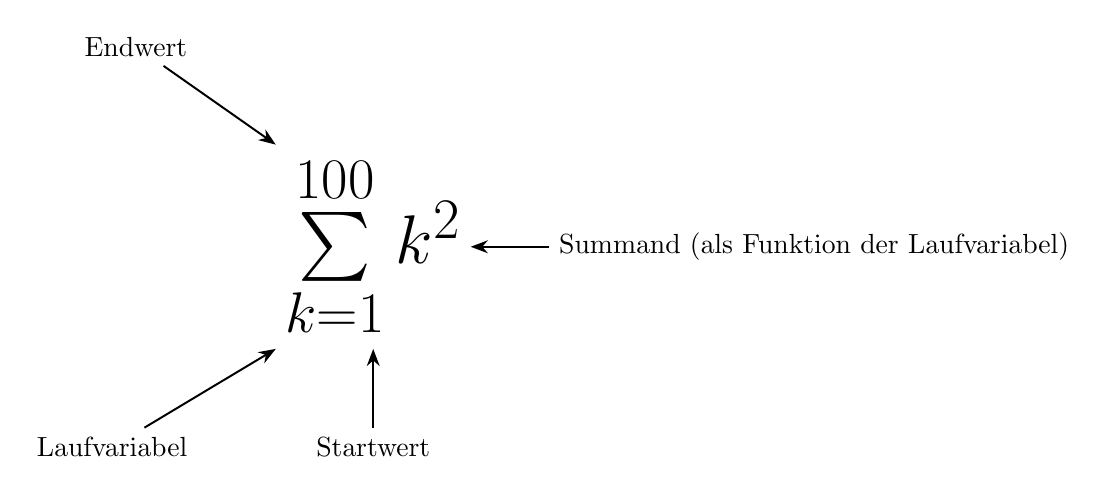
\begin{tikzpicture}
    \node (s) {\Huge{$\sum\limits_{k=1}^{100} k^2$}};
    \node[above left=of s] (end) {Endwert};
    \node[below left=of s] (index) {Laufvariabel};
    \node[below= of s] (start) {Startwert};
    \node[right= of s] (funktion) {Summand (als Funktion der
    Laufvariabel)};

    \draw[myarrow] (end) -- (s.north west);
    \draw[myarrow] (index) -- (s.south west);
    \draw[myarrow] (start) -- (s);
    \draw[myarrow] (funktion) -- (s);
\end{tikzpicture}
\end{document}
